\chapterimage{chapter_2.png}
\chapter{数据结构}

\begin{center}
    \pgfornament[width=0.36\linewidth,color=lsp]{88}
\end{center}

\section{单链表}
\lstinputlisting[style=cpp]{code/data_structure/linked_list/single.cpp}

\section{双链表}
\begin{figure}[H] %H为当前位置,!htb为忽略美学标准,htbp为浮动图形
\centering %图片居中
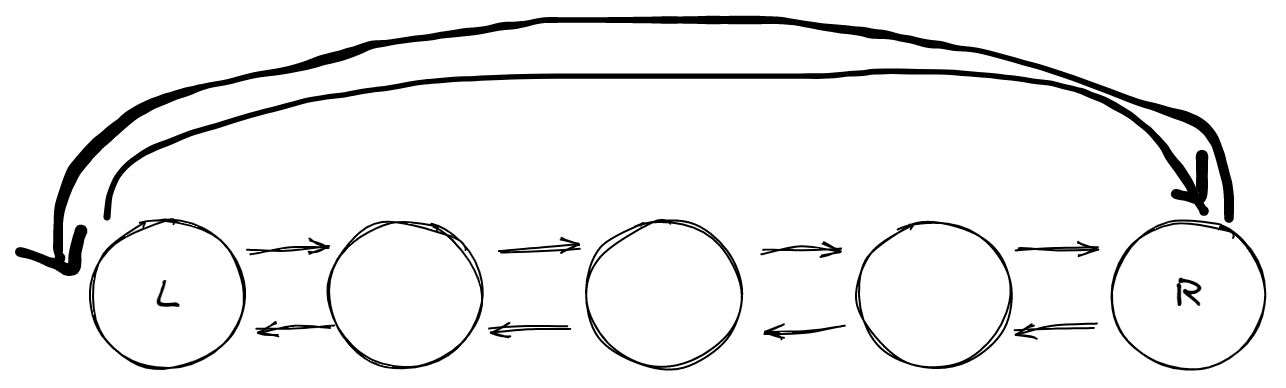
\includegraphics[width=0.9\textwidth]{images_content/4.png} %插入图片,[]中设置图片大小,{}中是图片文件名
\caption{双链表示意} %最终文档中希望显示的图片标题
\end{figure}

\lstinputlisting[style=cpp]{code/data_structure/linked_list/double.cpp}

\section{栈}
\subsection{数组模拟栈}
使用数组模拟栈的代码如下(stl中有现成的栈的实现):
\lstinputlisting[style=cpp]{code/data_structure/stack/normal.cpp}

\subsection{单调栈}
常见模型:找出每个数左边离它最近的比它大/小的数
\lstinputlisting[style=cpp]{code/data_structure/stack/monotonic.cpp}

\section{队列}
\subsection{普通队列}
\lstinputlisting[style=cpp]{code/data_structure/queue/normal.cpp}

\subsection{循环队列}
\lstinputlisting[style=cpp]{code/data_structure/queue/circular.cpp}

\subsection{单调队列}
常见模型:找出滑动窗口中的最大值/最小值
\lstinputlisting[style=cpp]{code/data_structure/queue/monotonic.cpp}

\section{Tire树}
字典树,是一种空间换时间的数据结构,又称Trie树、前缀树,是一种树形结构(字典树是一种数据结构),典型用于统计、排序、和保存大量字符串。所以经常被搜索引擎系统用于文本词频统计。它的优点是:利用字符串的公共前缀来减少查询时间,最大限度地减少无谓的字符串比较,查询效率比哈希树高。
\begin{figure}[H]
\centering
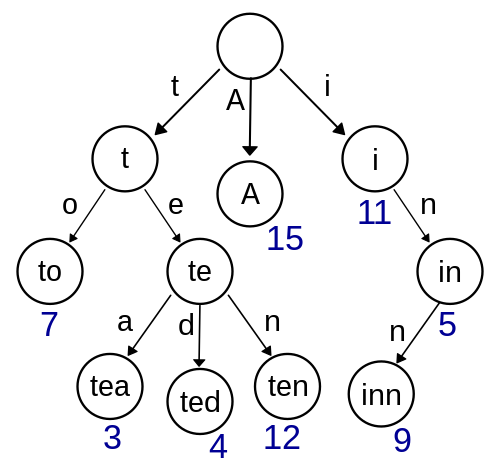
\includegraphics[width=0.7\textwidth]{images_content/5.png}
\caption{Tire树}
\end{figure}

\lstinputlisting[style=cpp]{code/data_structure/tire.cpp}


\section{并查集 DSU/UF}
\textbf{DSU}: Disjoint Set Union; \textbf{UF}: Union Find
并查集是一种树形的数据结构,顾名思义,它用于处理一些不交集的 合并 及 查询 问题。 它支持两种操作: 

\begin{itemize}
    \item 合并(Union):将两个子集合并成一个集合。
    \item 查找(Find):确定某个元素处于哪个子集;
\end{itemize}

\lstinputlisting[style=cpp]{code/data_structure/union_find.cpp}

\ifshowLink
讲解: \href{https://labuladong.github.io/algo/2/22/53/}{https://labuladong.github.io/algo/2/22/53/}\\
相关题目:
    \begin{enumerate}
        \item LeetCode 990. Satisfiability of Equality Equations: \href{https://leetcode.cn/problems/satisfiability-of-equality-equations/}{https://leetcode.cn/problems/satisfiability-of-equality-equations/}
    \end{enumerate}
\fi